\documentclass[a4paper, 12pt, final, garamond]{book}
\usepackage{cours-preambule}

\raggedbottom

\makeatletter
\renewcommand{\@chapapp}{M\'ecanique -- chapitre}
\makeatother

\begin{document}
\setcounter{chapter}{2}

\chapter{TD application~: mouvements courbes}

\section{Projection de vecteurs}
\begin{enumerate}
    \item Exprimer $\vfo$ dans la base $(\ux,\uz)$ en fonction de $v_0$ et
        $\a$.
        \begin{center}
            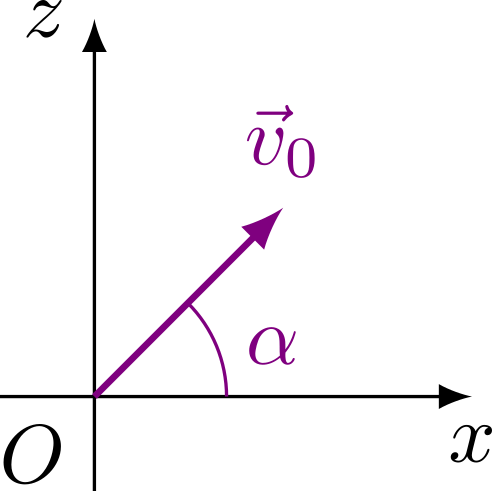
\includegraphics[scale=1]{vec_a}
        \end{center}
    \item Exprimer $\Nf$ et $\Tf$ dans la base $(\ux,\uz)$ en fonction de $N$,
        $T$ et $\a$.
        \begin{center}
            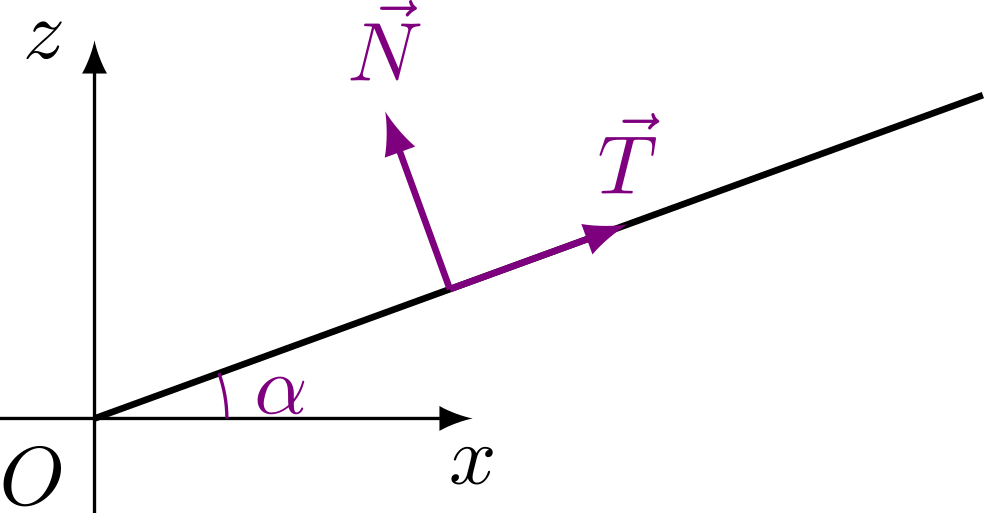
\includegraphics[scale=1]{vec_b}
        \end{center}
    \item Exprimer $\Pf$ et $\Tf$ dans la base $(\er,\et)$ en fonction de $m$,
        $g$, $T$ et $\tt$.
        \begin{center}
            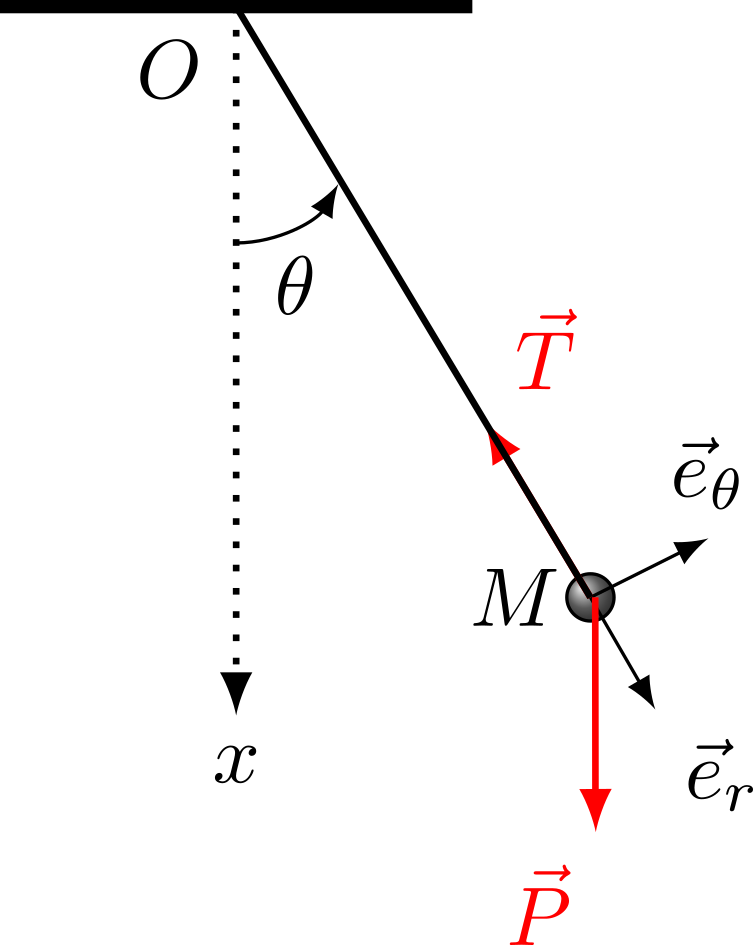
\includegraphics[scale=1]{vec_c}
        \end{center}
    \item \textbf{Équilibre plan incliné}
        À l'équilibre des forces, on a
        \[\Nf + \Tf + \Pf = \of\]
        Projeter le poids dans la base inclinée et exprimer les normes de $\Tf$
        et $\Nf$ en fonction de $m$, $g$ et $\a$.
        \begin{center}
            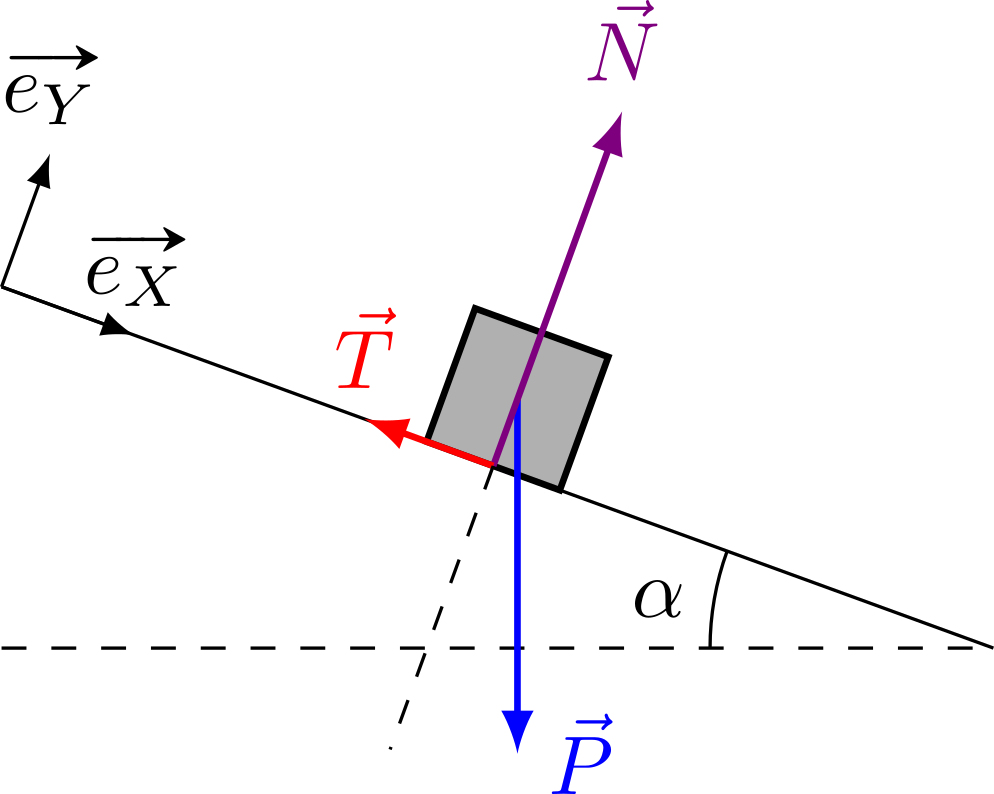
\includegraphics[scale=1]{vec_d}
        \end{center}
    \item \textbf{Équilibre hamac}
        À l'équilibre des forces, on a
        \[\Ff_g + \Ff_d + \Pf = \of\]
        Projeter les vecteurs $\Ff_g$ et $\Ff_d$ dans la base $(\ux,\uy)$ avec
        $\ux$ parallèle au sol vers la droite et $\uy$ vertical ascendant. En
        déduire la norme littérale de ces deux vecteurs. On prend $m =
        \SI{60}{kg}$, $\a = \ang{45}$ et $\beta = \ang{60}$.
        \begin{center}
            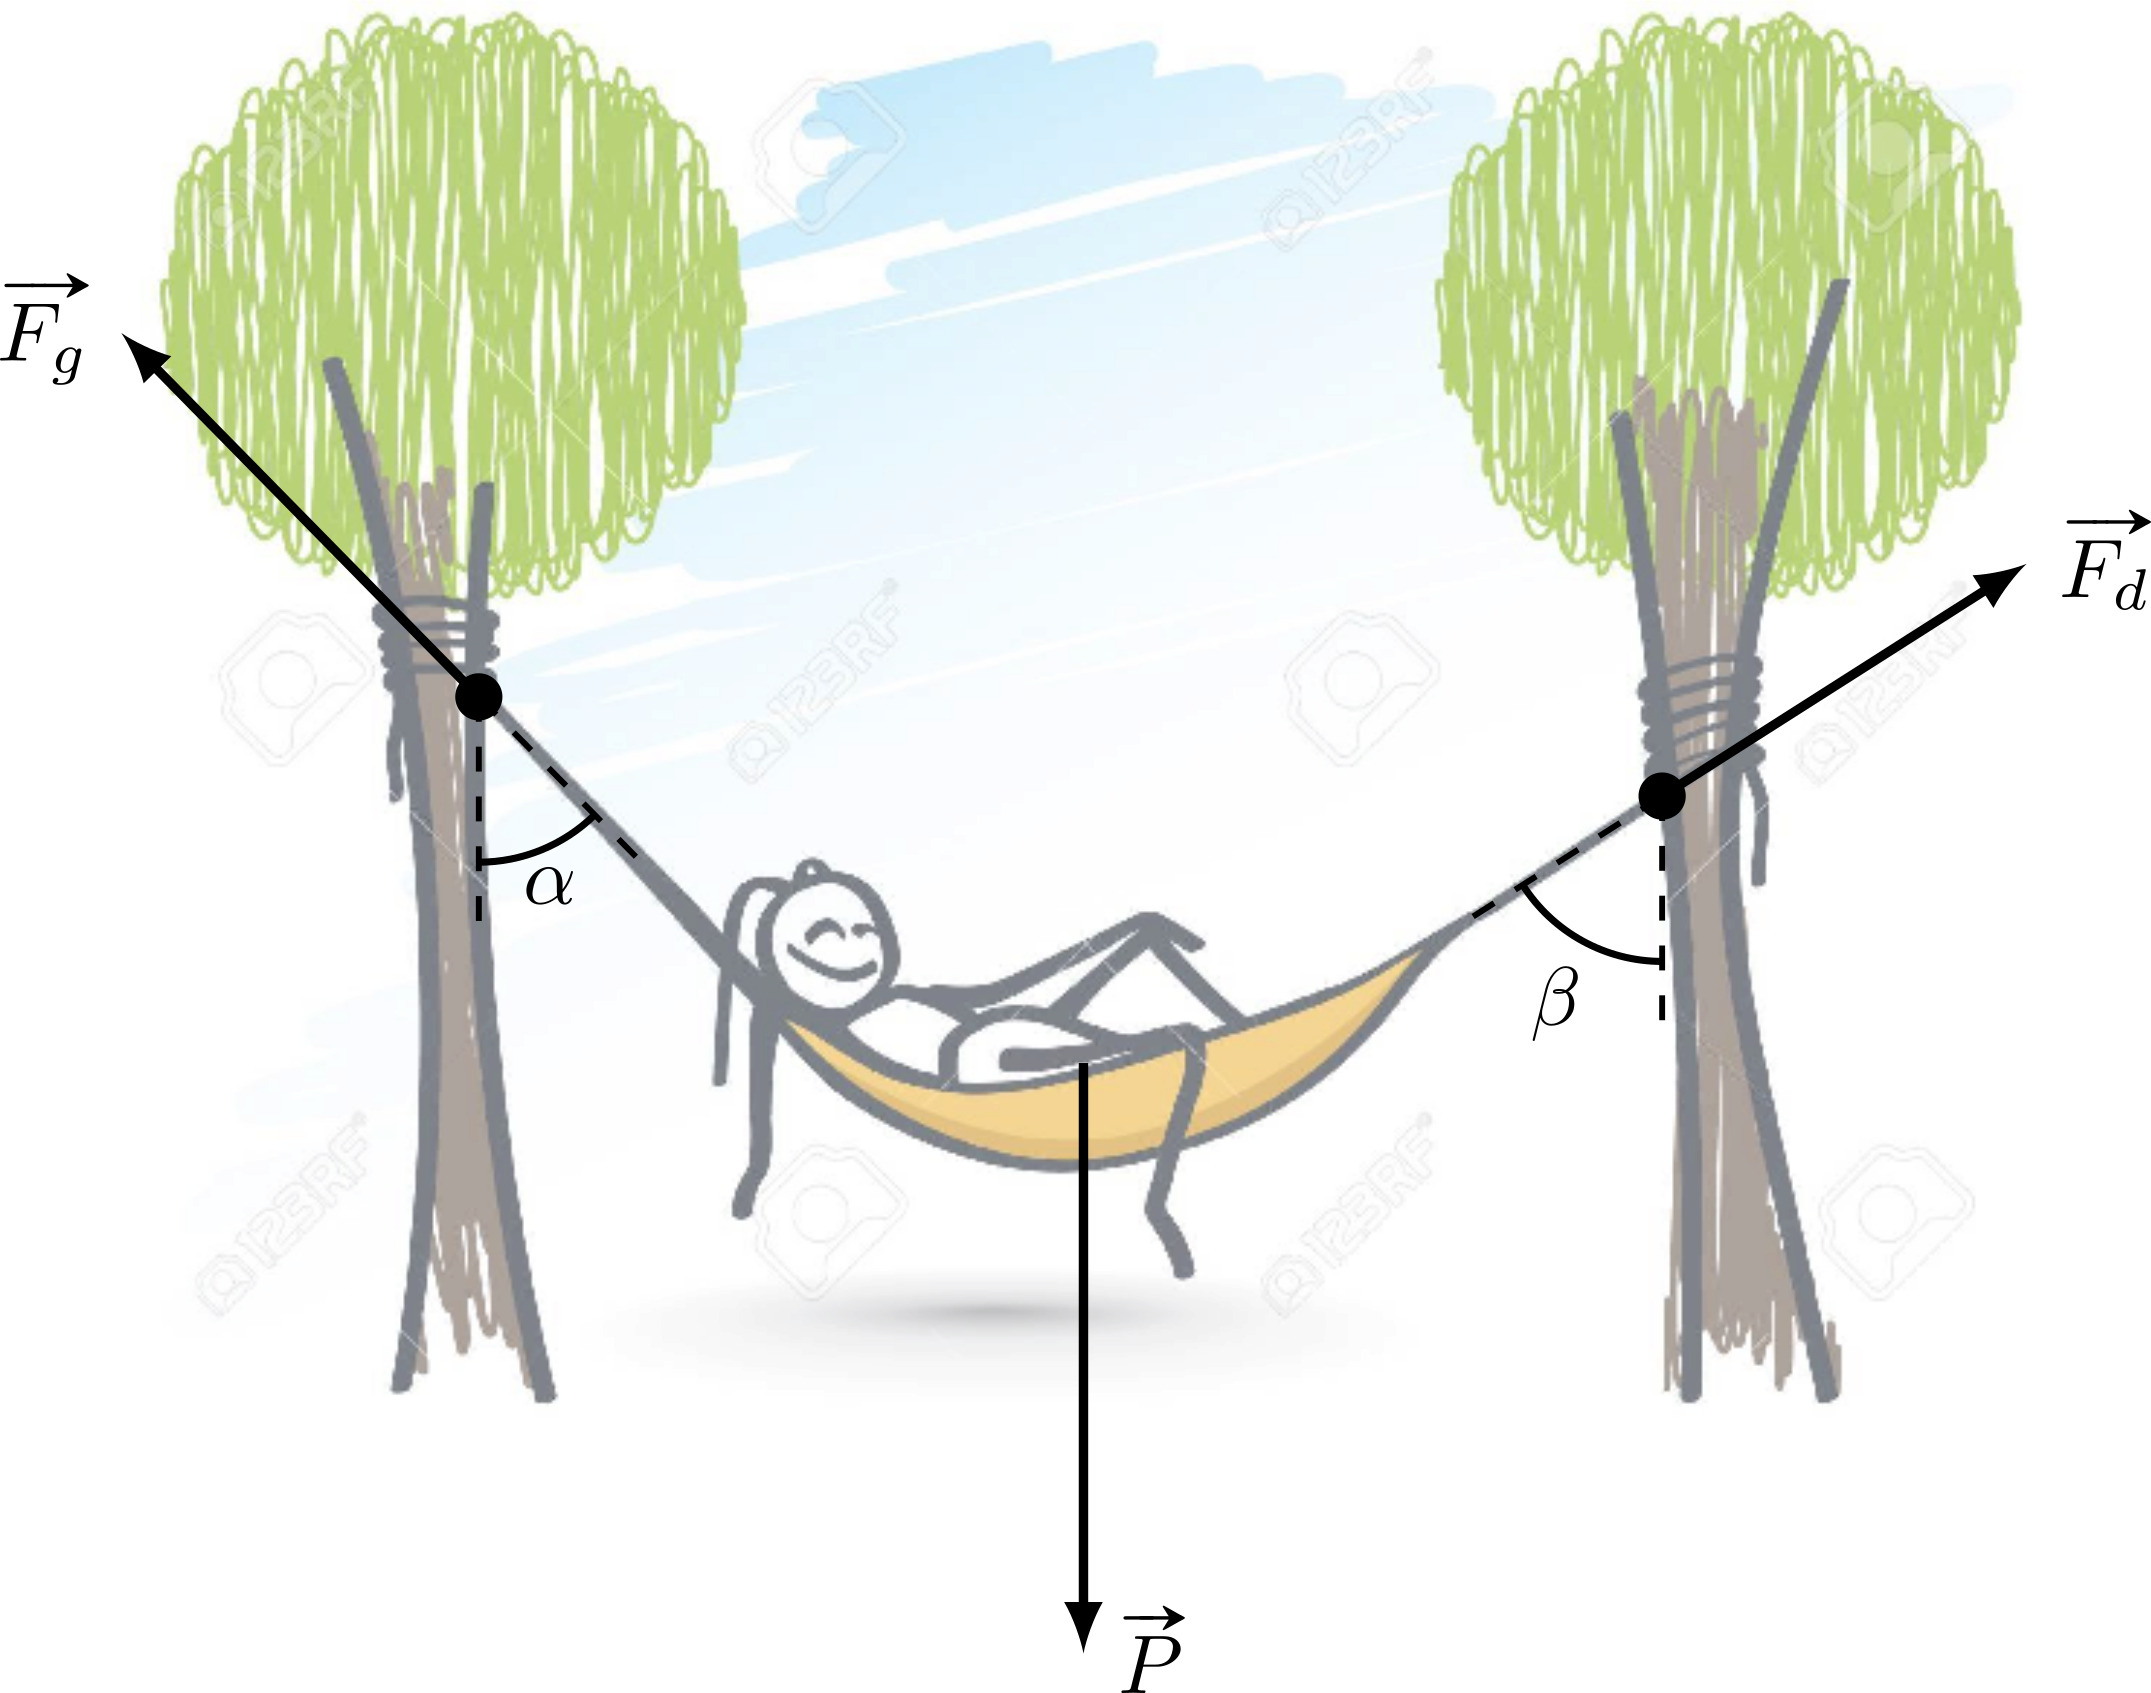
\includegraphics[scale=.7]{vec_e}
        \end{center}
\end{enumerate}

\section{Masse du Soleil}
La Terre subit de la part du Soleil la force d'attraction gravitationnelle~:
\[
    \Ff_g = -\Gc \frac{M_TM_S}{R^2}\ur
    \qMath{où}
    \Gc = \SI{6.67e-11}{SI}
\]
avec $\ur$ le vecteur unitaire allant du Soleil vers la Terre. La Terre tourne
autour du Soleil en décrivant un cercle de rayon $R = \SI{149.6e6}{km}$.
Déterminer la masse du Soleil.

\section{Oscillations d'un anneau sur un cerceau}
\hspace*{-0.75cm}
\begin{minipage}{0.70\linewidth}
    Un cerceau de centre O et de rayon $R$ est maintenu dans un plan vertical, et un
    anneau de masse $m$ assimilé à un point matériel M peut glisser sans frottements
    le long de ce cerceau.
    \begin{enumerate}
        \item Qu'est-ce que l'hypothèse «~sans frottements~» implique pour la
            réaction du cerceau sur l'anneau~?
        \item Écrire le PFD appliqué à l'anneau et le projeter dans une base
            adaptée.
        \item En déduire l'équation différentielle régissant le mouvement.
    \end{enumerate}
    On se place dans l'approximation des petits angles ($\abs{\tt} < \tt_0 =
    \ang{20}$). Initialement, l'anneau est situé à la verticale en-dessous de O et
    il est lancé vers la droite, avec une vitesse initiale de norme $v_0$.
\end{minipage}
\hfill
\begin{minipage}{0.25\linewidth}
    \begin{center}
        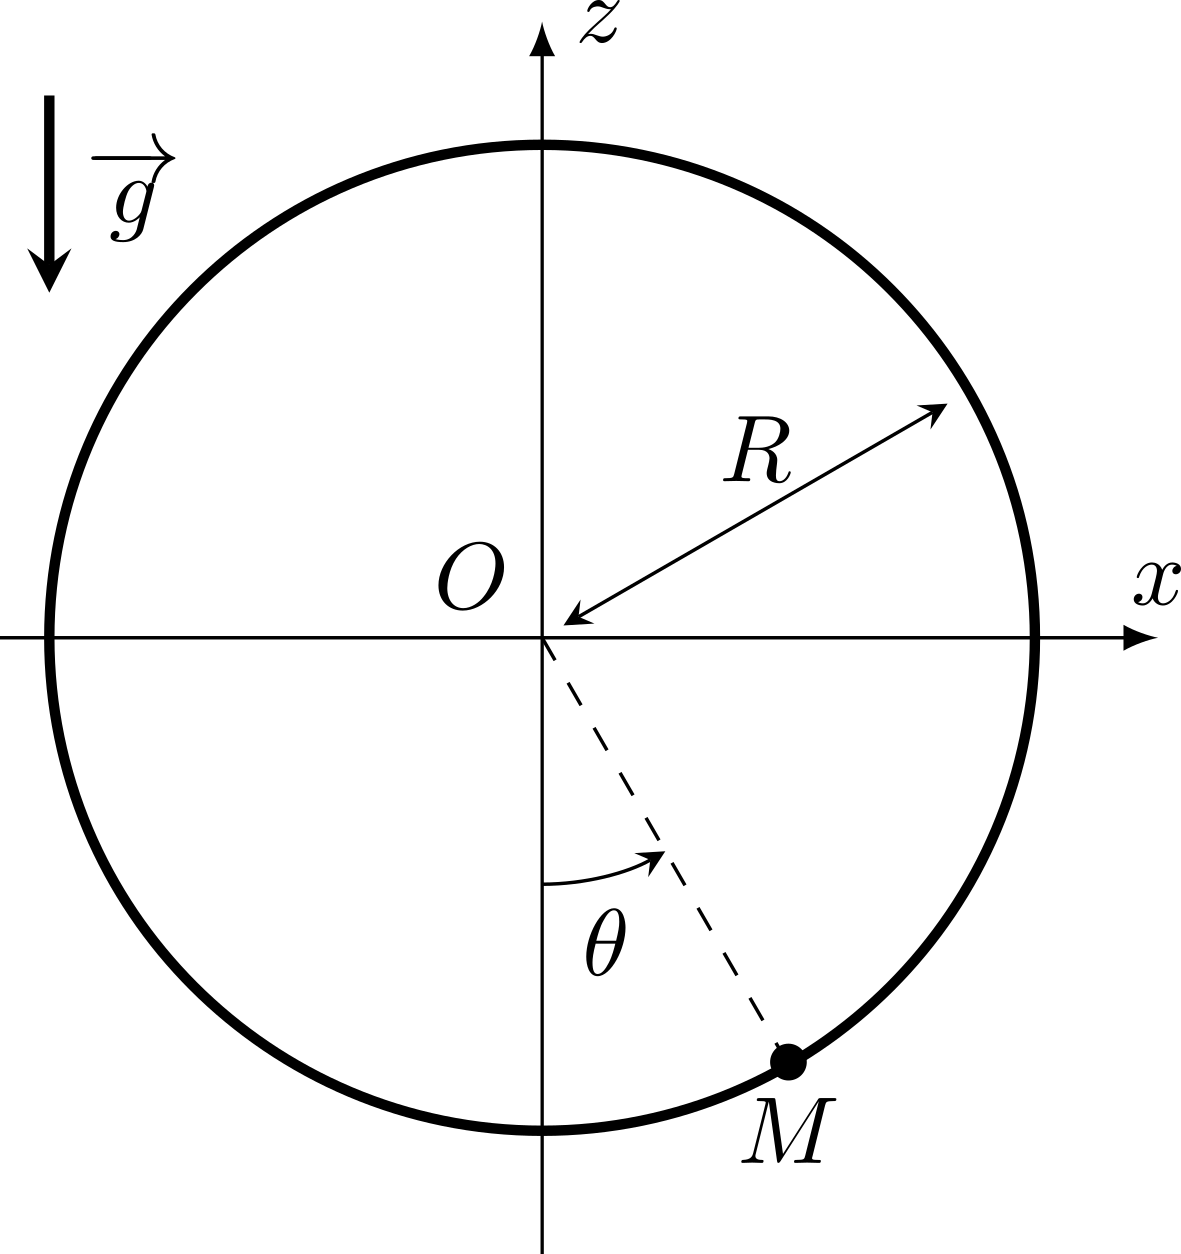
\includegraphics[width=\linewidth]{anneau_cerceau-plain}
    \end{center}
\end{minipage}
\begin{enumerate}[start=4]
    \item En déduire l'équation horaire du mouvement.
    \item À quelle condition sur $v_0$ l'approximation des petits angles
        est-elle vérifiée~?
\end{enumerate}

\section{Mouvement hélicoïdal}
Un point matériel M a pour équations horaires en coordonnées cylindriques~:
\[
    \left\{
        \begin{aligned}
            r(t)   & = R\\
            \tt(t) & = \wt\\
            z(t)   & = \a t
        \end{aligned}
    \right.
    \qavec
    (\a,\w)
    \quad
    \text{des constantes}
\]
\begin{enumerate}
    \item Exprimer le vecteur vitesse et le vecteur accélération dans la base
        cylindrique.
    \item Dessiner l'allure de la trajectoire.
    \item Déterminer $h$ le pas de l'hélice, c'est-à-dire la distance selon
        l'axe (O$z$) dont sont séparés deux points successifs de la trajectoire
        correspondant à un même angle $\tt$ (modulo $2\pi$).
    \item Ce mouvement est-il uniforme~? À quelle condition est-il circulaire~?
    \item Déterminer les coordonnées cartésiennes de ce mouvement.
\end{enumerate}


\end{document}
